% =====================================================================
% Journée 2 — Section 3 (S7) : TP Symfony Avis-Clients
% Compte rendu individuel — différences observées avec Django
% Compilation : tectonic Devoir_J2_S7_Symfony.tex
% =====================================================================
\documentclass[11pt,a4paper]{article}

\usepackage[utf8]{inputenc}
\usepackage[T1]{fontenc}
\usepackage[french]{babel}
\usepackage{mathptmx}            % Times New Roman (texte + maths)
\usepackage[scaled=0.85]{helvet} % sans-serif assorti
\usepackage{courier}             % mono pour le code
\usepackage[margin=2cm]{geometry}
\usepackage{booktabs}
\usepackage{tabularx}
\usepackage{ragged2e}
\usepackage{enumitem}
\usepackage{titlesec}
\usepackage{xcolor}
\usepackage{listings}
\usepackage{graphicx}
\usepackage{float}
\usepackage{caption}
\usepackage{fancyhdr}
\usepackage{lastpage}

\captionsetup{font=small,labelfont=bf,skip=4pt}
\graphicspath{{./}{avis-clients/}{catalog-service/}}

% ---------- Couleurs sobres (noir & blanc) ----------
\definecolor{gristexte}{gray}{0.35}
\definecolor{codebg}{gray}{0.96}

% ---------- En-tête / pied de page ----------
\pagestyle{fancy}
\fancyhf{}
\fancyfoot[C]{\small\itshape\color{gristexte}Page \thepage}
\renewcommand{\headrulewidth}{0.4pt}
\renewcommand{\footrulewidth}{0pt}

% ---------- Style des titres ----------
\titleformat{\section}{\normalfont\Large\bfseries}{\thesection.}{0.5em}{}[\titlerule]
\titleformat{\subsection}{\normalfont\large\bfseries}{}{0em}{}
\titlespacing*{\section}{0pt}{14pt}{8pt}
\titlespacing*{\subsection}{0pt}{10pt}{4pt}

% ---------- Listes plus compactes ----------
\setlist[itemize]{leftmargin=1.4em,itemsep=2pt,topsep=3pt}

% ---------- Bloc de code ----------
\lstset{
  basicstyle=\ttfamily\small,
  backgroundcolor=\color{codebg},
  frame=none,
  framexleftmargin=4pt,
  xleftmargin=4pt,
  breaklines=true,
  showstringspaces=false,
  columns=fullflexible,
}

% Colonne X justifiée pour tabularx
\newcolumntype{Y}{>{\RaggedRight\arraybackslash}X}
% Colonne p à largeur fixe, alignée à gauche SANS césure (mots gardés entiers)
\newcolumntype{P}[1]{>{\RaggedRight\arraybackslash\hyphenpenalty=10000\exhyphenpenalty=10000}p{#1}}

\setlength{\parindent}{0pt}
\setlength{\parskip}{4pt}
\setlength{\emergencystretch}{2.5em}

\begin{document}

% =====================================================================
% TITRE
% =====================================================================
\thispagestyle{empty}
\begin{center}
  {\LARGE\bfseries Journée 2}\\[4pt]
  {\large\bfseries Architecture Micro-services}\\[6pt]
  {\normalsize\itshape Section 3 \textperiodcentered{} TP Symfony Avis-Clients (S7)}\\[6pt]
\end{center}

\vspace{4pt}
\hrule
\vspace{8pt}

Nom / Prénom : DANILO Elouan

\vspace{6pt}

% Numérotation du devoir global conservée : cette section est la 3.
\setcounter{section}{2}
\section{TP Symfony Avis-Clients, différences avec Django}

Le service \textbf{Avis-Clients} est codé en \textbf{Symfony~7} avec \textbf{API~Platform}. Il expose une entité \texttt{Review} avec un CRUD complet auto-généré, de la validation, un appel HttpClient au Catalogue, des tests PHPUnit et une documentation Swagger gratuite. La base est \textbf{MariaDB} (contre PostgreSQL pour le Catalogue), ce qui démontre le polyglottisme de persistance.

\subsection{La \og magie\fg{} d'API Platform}

Une seule annotation \texttt{\#[ApiResource]} sur l'entité génère tout le CRUD REST \textbf{et} la doc OpenAPI. La validation se déclare par des attributs posés directement sur les propriétés.

\begin{lstlisting}[language=PHP]
#[ORM\Entity(repositoryClass: ReviewRepository::class)]
#[ApiResource(operations: [
    new GetCollection(), new Get(),
    new Post(processor: ReviewPersistProcessor::class),
    new Patch(processor: ReviewPersistProcessor::class),
    new Delete(),
])]
class Review
{
    #[Assert\Range(min: 1, max: 5, notInRangeMessage: 'Note entre {{ min }} et {{ max }}.')]
    private ?int $rating = null;

    #[Assert\NotBlank]
    #[Assert\Length(min: 5, max: 1000)]
    private ?string $comment = null;

    #[Assert\Positive]
    private ?int $productId = null;
    // ... author, createdAt
}
\end{lstlisting}

API~Platform expose alors automatiquement cinq opérations REST, à savoir \texttt{GET /api/reviews} (liste paginée), \texttt{POST /api/reviews} (création), \texttt{GET /api/reviews/\{id\}} (détail), \texttt{PATCH /api/reviews/\{id\}} (modification) et \texttt{DELETE /api/reviews/\{id\}} (suppression), le tout documenté en OpenAPI.

\subsection{Appel inter-services avec HttpClient et State Processor}

La vérification du produit est branchée dans un \textbf{State Processor} qui décore le \emph{persist} de Doctrine. Avant d'écrire, on interroge le Catalogue via le \textbf{HttpClient} de Symfony.

\begin{lstlisting}[language=PHP]
public function process(mixed $data, Operation $op, array $uriVars = [], array $ctx = []): mixed
{
    if ($data instanceof Review && !$this->catalogue->productExists($data->getProductId())) {
        throw new HttpException(422, 'Produit inexistant : aucun produit ... dans le Catalogue.');
    }
    return $this->persistProcessor->process($data, $op, $uriVars, $ctx);
}
\end{lstlisting}

\subsection{Tableau comparatif Django/DRF $\leftrightarrow$ Symfony/API~Platform}

\begin{tabularx}{\textwidth}{@{}P{3.4cm} Y Y@{}}
\toprule
\textbf{Thème} & \textbf{Django / DRF} & \textbf{Symfony / API~Platform} \\
\midrule
Génération API & ViewSet + Serializer + routeur à écrire & \texttt{\#[ApiResource]} $\rightarrow$ CRUD auto \\[3pt]
Documentation & drf-spectacular à configurer & Swagger \textbf{gratuite} sur \texttt{/api/docs} \\[3pt]
ORM & Django ORM & Doctrine (attributs \texttt{\#[ORM]}) \\[3pt]
Validation & \texttt{validate\_*} du serializer & Attributs \texttt{\#[Assert\textbackslash...]} \\[3pt]
Réponses & JSON simple & JSON-LD / Hydra (HATEOAS) \\[3pt]
Erreurs & détail DRF (400) & RFC 7807 (\texttt{/api/errors/422}) \\[3pt]
Appels sortants & \texttt{requests} & Symfony HttpClient \\[3pt]
Dépendances & pip / requirements.txt & Composer / composer.json \\[3pt]
Brique de code & \og app\fg{} Django & \og bundle\fg{} Symfony \\[3pt]
Hook d'écriture & \texttt{perform\_create()} & State Processor \\
\bottomrule
\end{tabularx}

\subsection{Tests}

\textbf{8 tests PHPUnit} passent (\texttt{WebTestCase} pour l'API et \texttt{KernelTestCase} pour la validation). Ils couvrent la liste, la création 201, le produit inexistant 422, la note hors bornes 422 et le commentaire vide 422. Le Catalogue est remplacé par un double de test pour ne pas dépendre du Django réel.

\subsection{Difficultés rencontrées et solutions}

Le code du service étant fourni, l'essentiel du travail a porté sur la mise en route de l'environnement et la résolution des problèmes de configuration.

\begin{tabularx}{\textwidth}{@{}P{5.6cm} Y@{}}
\toprule
\textbf{Difficulté} & \textbf{Solution mise en place} \\
\midrule
PHP, Composer et le Symfony CLI absents de la machine. & Installation de \textbf{PHP~8.3 portable} + \textbf{Composer} en espace utilisateur (sans droits administrateur), ajout au \texttt{PATH}. \\[4pt]
Composer refuse d'installer Symfony 7.1 (avis de sécurité). & Montée de version en \textbf{Symfony~7.4 / API~Platform~4.2}~; adaptation de la clé de config \texttt{docformats} $\rightarrow$ \texttt{docs\_formats}. \\[4pt]
Composer ne décompresse pas les paquets (\texttt{The zip extension is missing}). & Activation de \texttt{extension=zip} dans \texttt{php.ini}. \\[4pt]
La Swagger UI ne s'affiche pas (page cassée, logo absent, CSS/JS en 404). & (1)~installation de \texttt{twig-bundle} (template de la doc manquant)~; (2)~format \texttt{html} remis dans \texttt{formats}~; (3)~routeur \texttt{public/router.php} pour servir les assets (sinon \texttt{php -S} les renvoie en \texttt{text/html}). \\[4pt]
\texttt{config/routes.yaml} pointe vers un dossier \texttt{src/Controller} inexistant. & Création du dossier (service API-only, sans contrôleur). \\[4pt]
Aucun serveur MariaDB installé en local. & Exécution sur \textbf{SQLite} via \texttt{.env.local} (et \texttt{.env.test.local} pour les tests)~; la configuration MariaDB du TP est conservée pour Docker. \\[4pt]
\texttt{assertJsonContains()} indisponible en \texttt{WebTestCase}. & Décodage JSON manuel (\texttt{json\_decode}) puis assertions sur les champs. \\
\bottomrule
\end{tabularx}

\subsection{Livrables}

Le code, la collection Postman (\texttt{AvisClients.postman\_collection.json}) et le présent rapport sont versionnés dans le dépôt Git \texttt{https://github.com/Oasio/micro-service}. La documentation interactive Swagger est servie sur \texttt{/api/docs} (capture ci-dessous).

\begin{figure}[H]
  \centering
  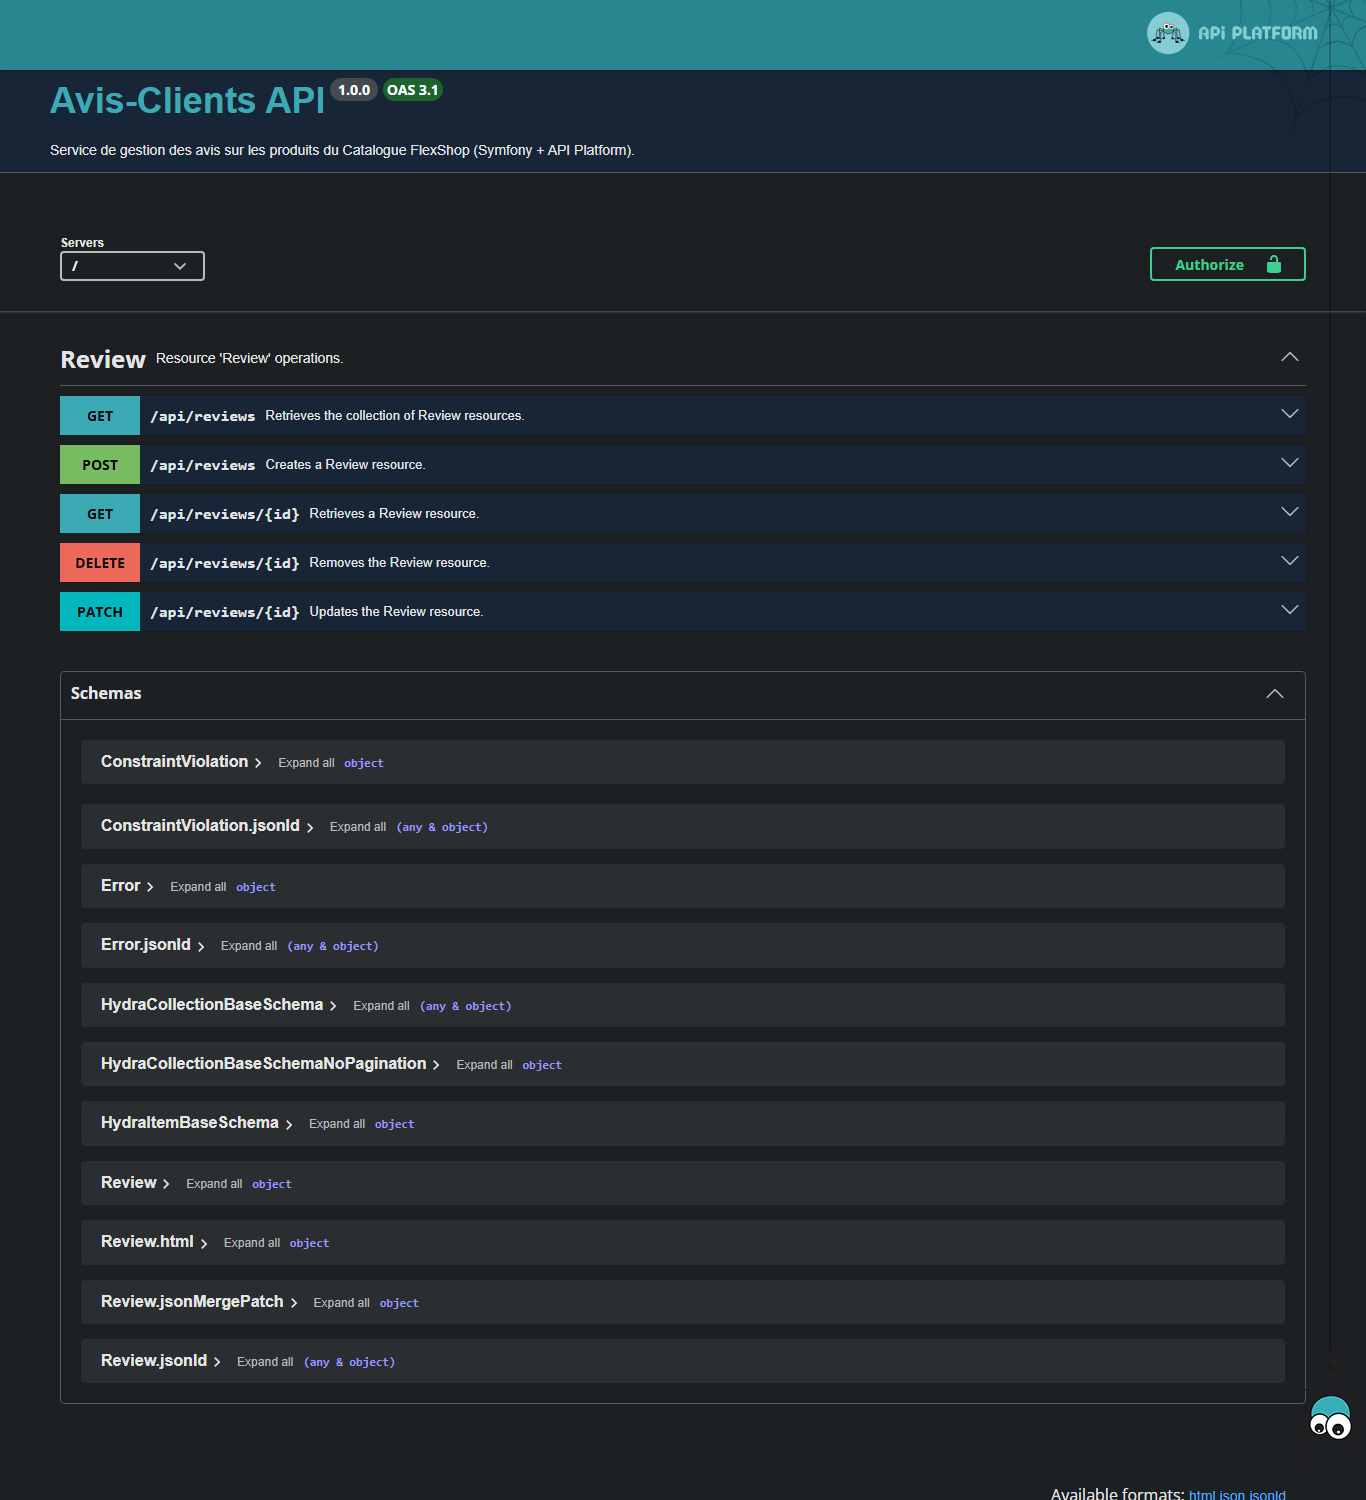
\includegraphics[width=0.82\textwidth]{swagger-avis.png}
  \caption{Swagger UI d'Avis-Clients sur \texttt{http://localhost:8001/api/docs}. Le CRUD complet est auto-généré par API~Platform, avec des schémas JSON-LD/Hydra.}
  \label{fig:swagger-avis}
\end{figure}

\end{document}
